
\ifnumequal{\value{rolldice}}{0}{
  \renewcommand{\va}{2}
}{
  \ifnumequal{\value{rolldice}}{1}{
    \renewcommand{\va}{3}
  }{
    \ifnumequal{\value{rolldice}}{2}{
      \renewcommand{\va}{4}
    }{
      \renewcommand{\va}{5}
    }
  }
} 

\POWER\va{4}\vb
\FRACTIONSIMPLIFY\vb{-12}\vm\vn
\ABSVALUE\vm\vo

\question[3] Find the area of the figure bounded by the $y-axis$ and the curve (see figure)
\[ x=y^2\cdot(y-\va) \]

\watchout

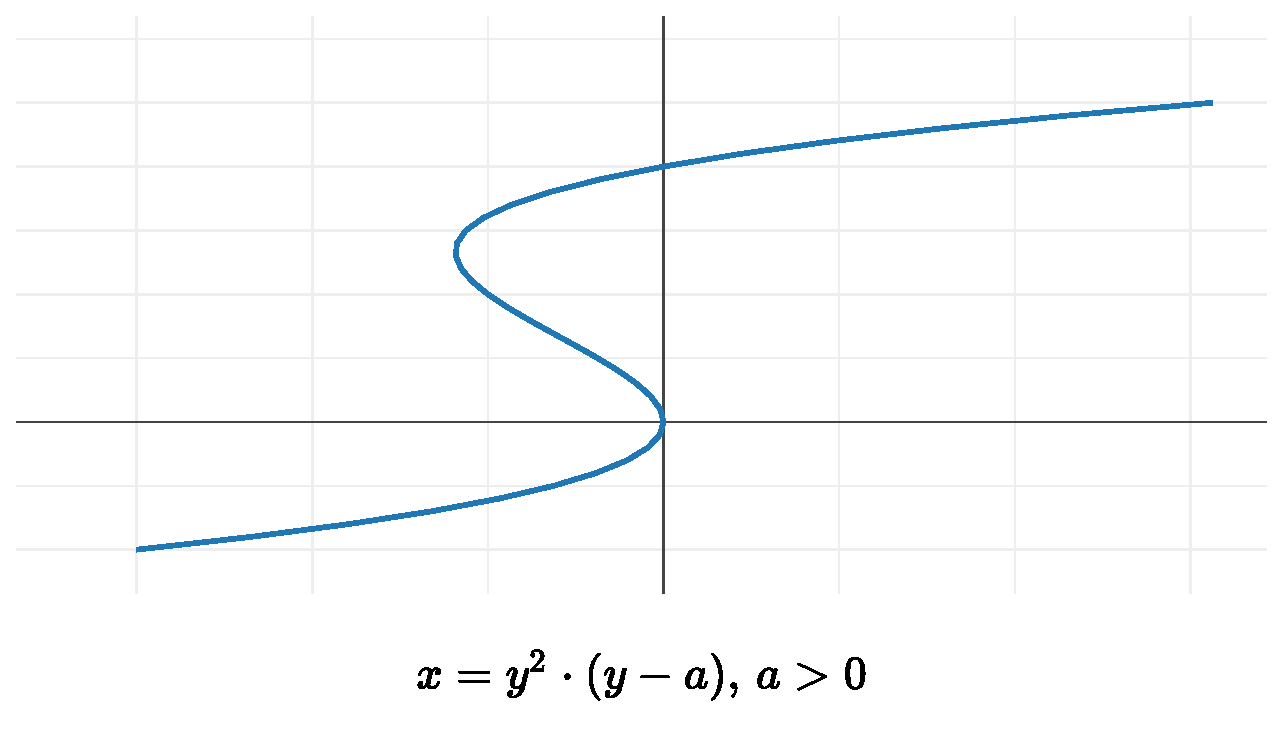
\includegraphics[width=300pt]{plotly.eps}

\begin{solution}[\halfpage]
  \textbf{Plotting $x=f(y)$}

  We are accustomed to seeing $y=f(x)$ - where $y$ is the dependent variable and 
  $x$ is the independent variable. 
  
  In this case, however, $x=f(y)$. To plot it (so that one can see the required area), 
  simply treat $y$ as the independent variable and $x$ as the dependent variable. 

  In other words, plot it like you would $y=x^2\cdot (x-\va)$ - but inter-change 
  the $y$ with the $x$. 

  \textbf{Back to the question $\ldots$}

  The required area $(A)$ is of the bulge between the points where $x=0$. In other words, where 
  \[ x = y^2\cdot(y-\va) = 0\implies y = 0, \va \]
  \begin{align}
     A &= \int_0^{\va} y^2\cdot(y-\va)\ud y 
     = \int_0^{\va}\left(y^3-\va y^2\right)\ud y \\
       &= \left[ \dfrac{y^4}{4} - \dfrac{\va y^3}{3}\right]_0^{\va} = \WRITEFRAC\vm\vn
  \end{align}
  
  As area cannot be negative, $A=\WRITEFRAC\vo\vn$
\end{solution}

\ifprintanswers
  \begin{codex}
    $\dfrac\vo\vn$
  \end{codex}
\fi
